\documentclass[french]{article}
\usepackage[T1]{fontenc}
\usepackage[utf8]{inputenc}
\usepackage{lipsum}
\usepackage{lmodern}
\usepackage{geometry}
\usepackage{babel}
\usepackage{graphicx}
\usepackage{lastpage}
\usepackage{ragged2e}
\usepackage[normalem]{ulem}
\usepackage{float}
\usepackage{import}
\usepackage{listings}

\setlength{\parindent}{0cm}

\geometry{
 	a4paper,
 	total={210mm,297mm},
 	left=20mm,
 	right=20mm,
 	top=25mm,
 	bottom=20mm,
}

\lstset{
    frame=single,
    breaklines=true,
    numbers=left,
    numbersep=6pt,
    tabsize=2,
    basicstyle=\small\sffamily
}

\usepackage{fancyhdr}
\pagestyle{fancy}

\lhead{Cotza Andrea \& Verdon Arthur}
\chead{}
\rhead{02.06.2016}
\cfoot{\thepage/\pageref{LastPage}}
\renewcommand{\headrulewidth}{0.4pt}
\renewcommand{\footrulewidth}{0.4pt}

\begin{document}
	\title{SER: Rapport laboratoire 3}
	\author{Cotza Andrea \& Verdon Arthur\\Prof. E. Lefrançois}
	\maketitle
    \vspace{5cm}
    \tableofcontents
    \newpage

    \section{Introduction}
    L'objectif de ce laboratoire consiste en la création d'un "site" permettant
    l'affichage des projections à partir d'un fichier XML et XSL (aussi appelé
    XSLT).

    \section{Modification éventuelle de la structure XML}
    Pas de modification particulière apportée à la structure XML dans ce labo.

    \section{Vision conceptuelle du programme}
    Le programme permettra de générer trois fichier HTML contenant chacun une
    présentation différente des films. Chaque film sera afficher avec ses détails
    contenu dans une div "collapse" (voir CSS/Bootrstrap).

    \section{Structure du programme}
    \subsection{XSL}
    La fichier XSL est découpé en plusieur templates décrit ci-dessous.
    \vspace{5}
    \\\\le premier des templates permet l'affichage des différents films et peut
    être appliqué dès que l'on veut afficher un film (il est d'ailleur appliquer
    dans les templates suivant).
    \lstinputlisting[language=xslt, firstline=225, lastline=231,numbers=none]{../Source/projections.xsl}
    \vspace{30}

    \\\\Trois autre template permettent de trier les films
    selon l'ordre voulu (par date de projection, par nom ou par classement/évaluation).
    Ces trois autre template applique le premier tempalte qui permet d'afficher la
    liste des films.
    \lstinputlisting[language=xslt, firstline=142, lastline=174,numbers=none]{../Source/projections.xsl}
    \vspace{30}

    \\\\Le dernier template permet d'afficher les acteurs dans le film et est appliqué
    dans le premier template s'occupant des films.
    \lstinputlisting[language=xslt, firstline=187, lastline=223,numbers=none]{../Source/projections.xsl}
    \vspace{30}

    \\\\Le XSL génère ensuite trois fichiers HTML chacun contenants un tri différent.
    \lstinputlisting[language=xslt, firstline=9, lastline=28,numbers=none]{../Source/projections.xsl}

    \subsection{CSS}
    Afin de gagner en rapidité de dévellopement, il a été choisi d'utiliser un
    framework CSS/Javascript pour le design de la page HTML (générer depuis le XSL et le XML).
    Ce framework s'appel Bootstrap et nous a permis d'avoir un design correct pour la page.
    Peu de code CSS ont donc été nécessaire c'est pourquoi celui-ci ne sera pas
    ajouté dans les annexes.

    \subsection{Javascript}
    Comme dit précédement un framework à été utilisé pendant ce labo donc peu de
    JS à été écrit (pour les même raisons il ne sera pas ajouté dans les annexes).

    \\ En complèment a Bootrstrap, nous avons utilisé JQuery (qui est nécessaire
    pour Bootstrap) et une petite librairie (qui utilise Boostrap) qui permet
    d'afficher des étoiles pour les critiques.

    \newpage
    \section{Resultats}
    Voici quelques captures d'écran présentant nos résultats
    \begin{center}

      \fbox{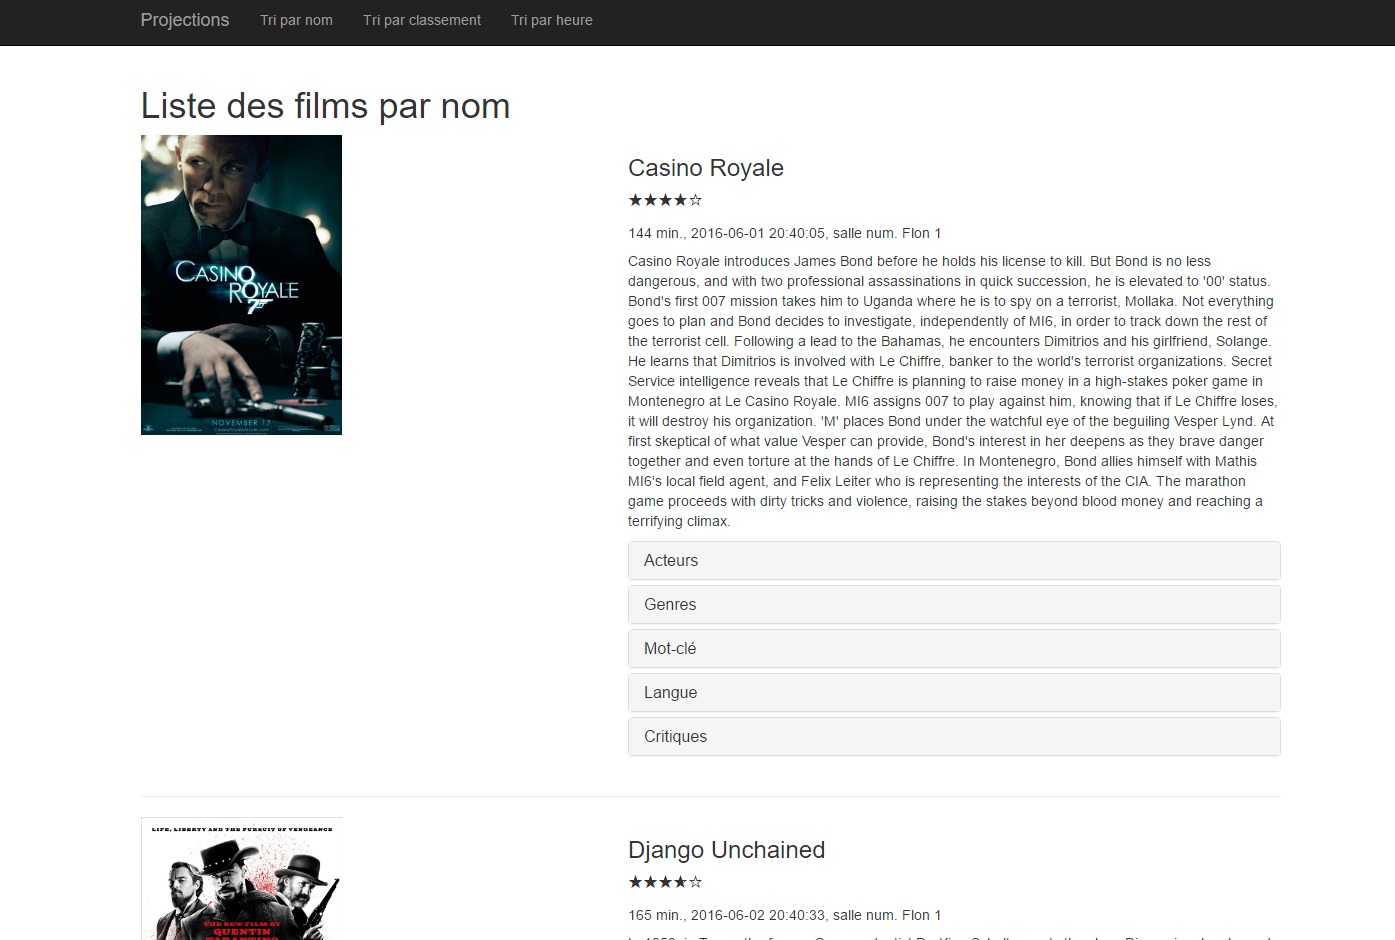
\includegraphics[height=200]{./img/resultat1.PNG}}
      \\\caption{Exemple de la page listant les films par noms}}
      \\\vspace{30}
      \fbox{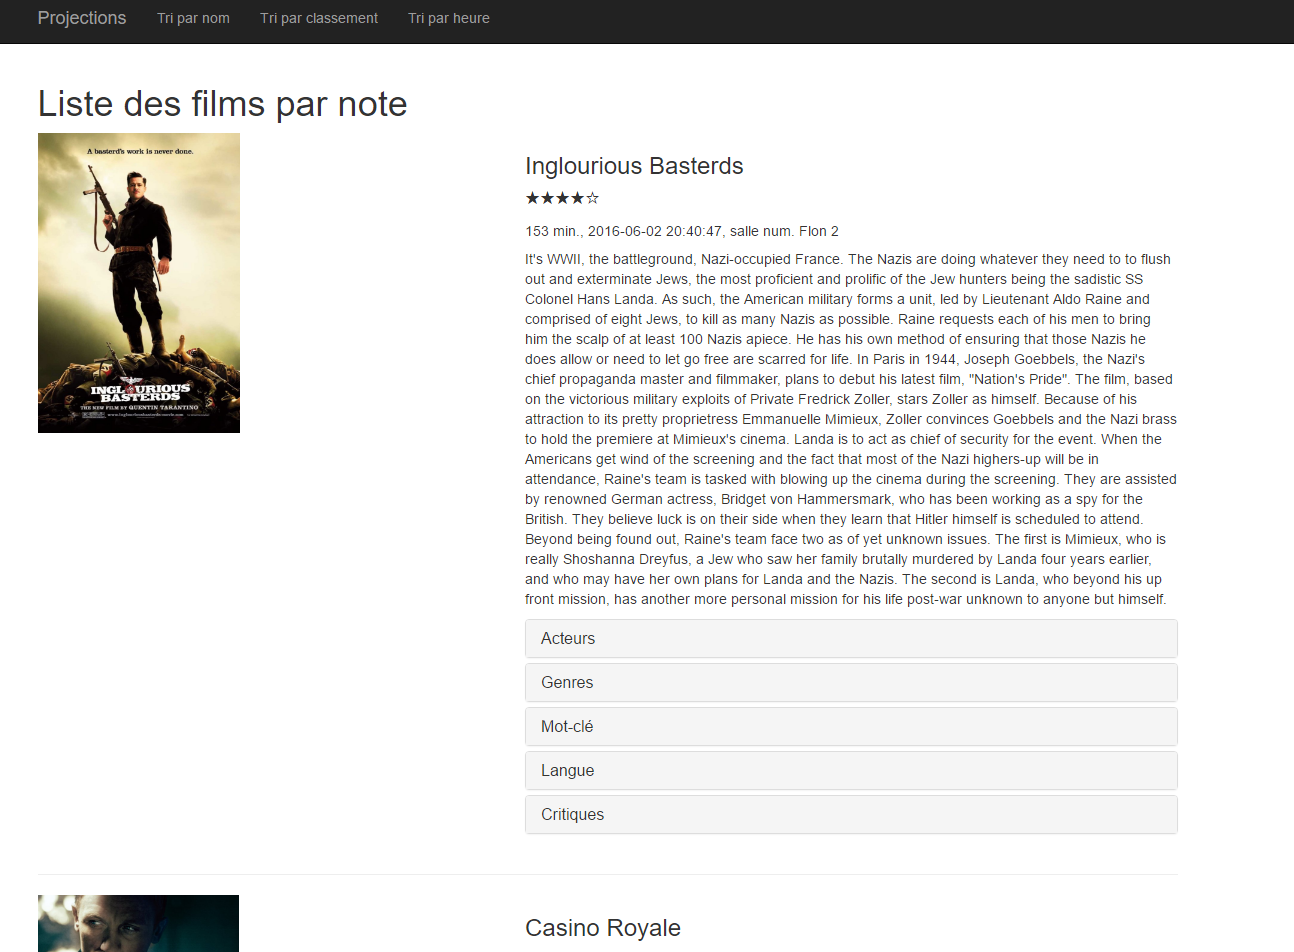
\includegraphics[height=200]{./img/resultat2.PNG}}
      \\\caption{Exemple de la page listant les films par note}
      \\\vspace{30}
      \fbox{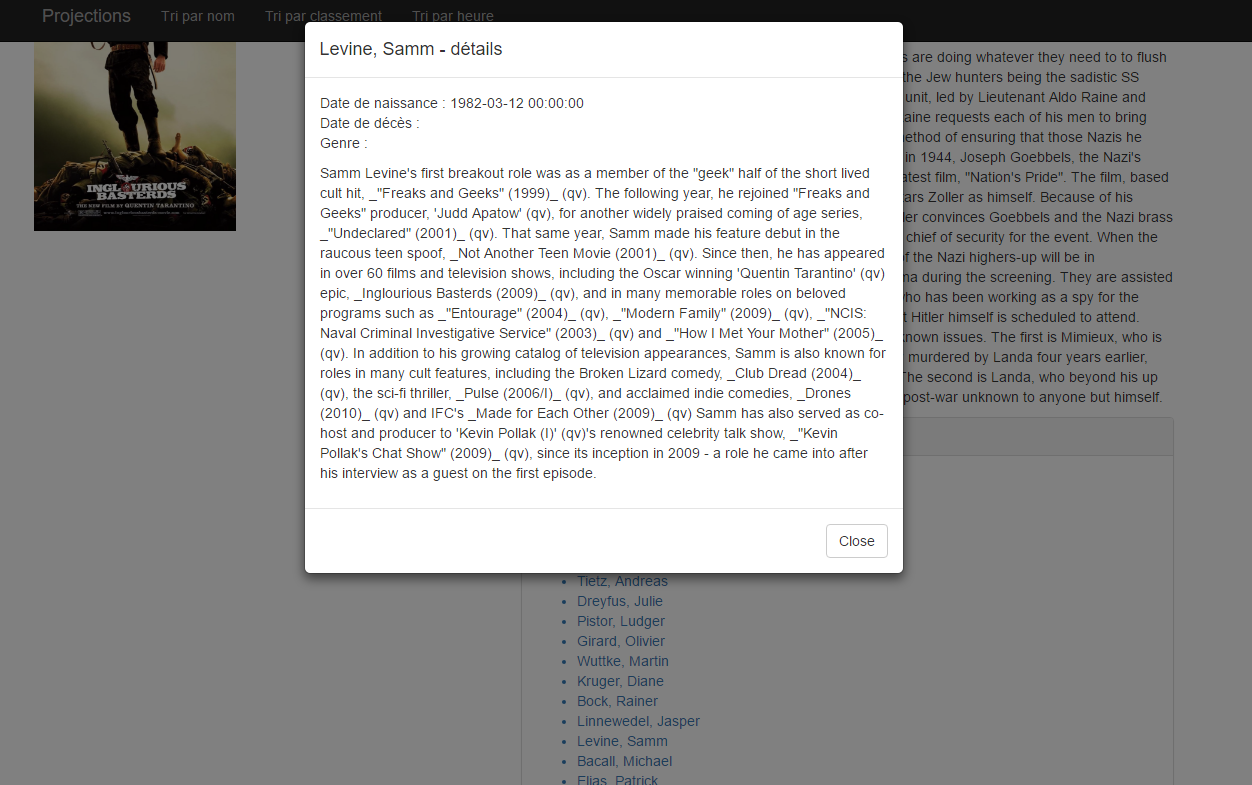
\includegraphics[height=200]{./img/resultat3.PNG}}
      \\\caption{Exemple d'affichage des détails d'un acteur}
      \\\vspace{30}
      \fbox{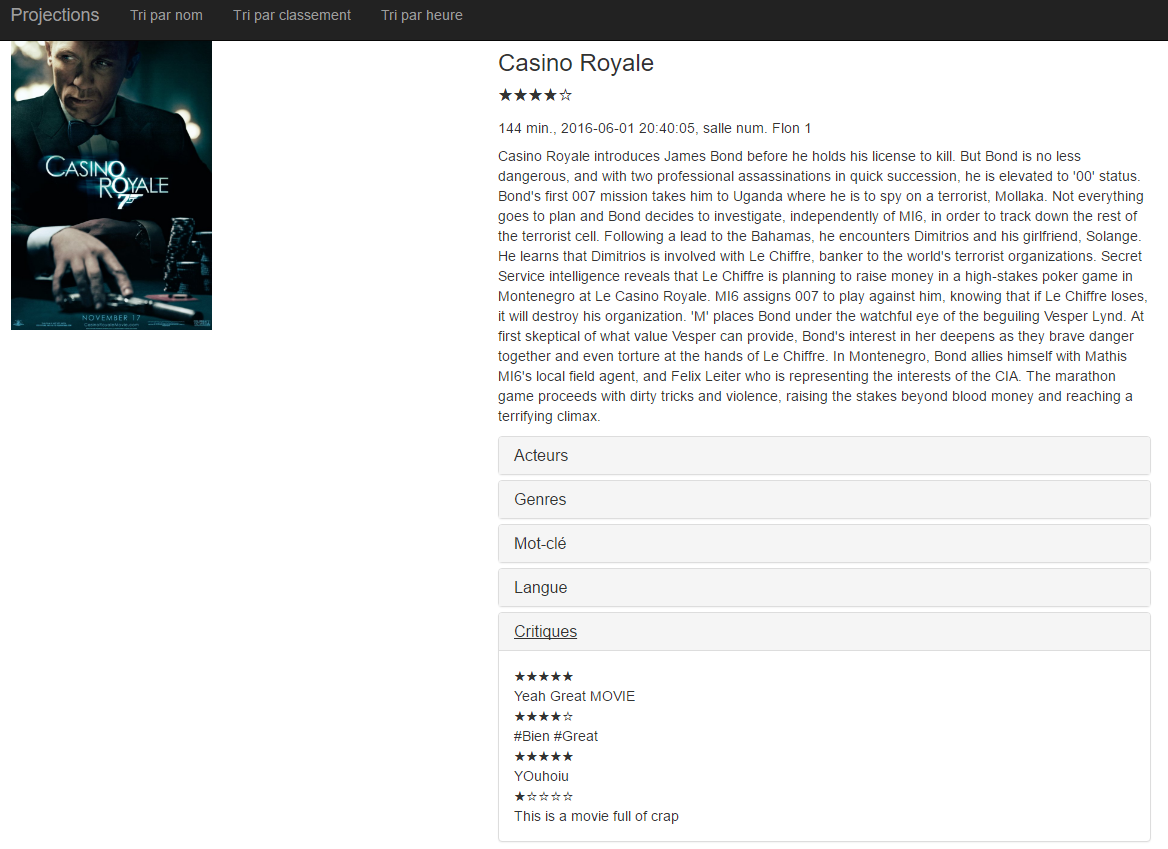
\includegraphics[height=200]{./img/resultat4.PNG}}
      \\\caption{Exemple d'affichage des différentes critiques d'un film}
    \end{center}


    \newpage
    \section{Comment obtenir ce résultat}
    Pour obtenir ce résultat il suffit de taper la commande suivante :\\
    \begin{lstlisting}[numbers=none]
      java -cp saxon9he.jar net.sf.saxon.Transform -s:{LE FICHIER CONTENANT LES PROJECTIONS}.xml -xsl:projections.xsl
    \end{lstlisting}

    \section{Conclusion}
    Dans ce labo nous avons pu constater que XSLT pouvait s'avérer utile dans le
    cas ou le contenu d'un fichier XML devrait être rendu présentable. Toutefois
    nous avons trouvé ce langage assez lourd d'utilisation pour la génération
    d'un HTML.

    \newpage

    \section{Annexe}
    \subsection{Code projections.xsl}
    \lstinputlisting[language=XSLT]{../Source/projections.xsl}

\end{document}
